\documentclass[format=sigconf]{acmart}
\usepackage[utf8]{inputenc}
\usepackage{geometry}
\usepackage{enumitem}
\usepackage{float}
\usepackage[labelfont=bf,textfont=md]{caption}
\usepackage{graphicx}
\usepackage{xcolor}
\usepackage{minted}
\usepackage{hyperref}
\usepackage[parfill]{parskip}
\usepackage[all]{hypcap}
\usemintedstyle[common-lisp]{default}
\newmintinline[code]{text}{}
\bibliographystyle{plainnat}

\hypersetup{
  colorlinks,
  linkcolor={red!50!black},
  citecolor={blue!50!black},
  urlcolor={blue!80!black}
}

\newlist{step}{enumerate}{10}
\setlist[step]{label*=\arabic*.,leftmargin=2em}

\acmConference[ELS’24]{the 17th European Lisp Symposium}
{May 6--7 2024}{Vienna, Austria}
\acmDOI{}
\setcopyright{rightsretained}
\copyrightyear{2024}

\begin{document}

\title{Convex Covering, a Refined Approach to Convex Decomposition of Collision Geometry}

\author{Jan ``Scymtym'' Moringen}
\email{jmoringe@techfak.uni-bielefeld.de}
\author{Yukari ``Shinmera'' Hafner}
\email{shinmera@tymoon.eu}
\affiliation{%
  \institution{Shirakumo.org}
  \city{Zürich}
  \country{Switzerland}
}

\begin{CCSXML}
  <ccs2012>
  <concept>
  <concept_id>10010147.10010371.10010396.10010398</concept_id>
  <concept_desc>Computing methodologies~Mesh geometry models</concept_desc>
  <concept_significance>500</concept_significance>
  </concept>
  <concept>
  <concept_id>10010147.10010371</concept_id>
  <concept_desc>Computing methodologies~Computer graphics</concept_desc>
  <concept_significance>500</concept_significance>
  </concept>
  <concept>
  <concept_id>10010405.10010469.10010474</concept_id>
  <concept_desc>Applied computing~Media arts</concept_desc>
  <concept_significance>100</concept_significance>
  </concept>
  </ccs2012>
\end{CCSXML}

\ccsdesc[500]{Computing methodologies~Mesh geometry models}
\ccsdesc[500]{Computing methodologies~Computer graphics}
\ccsdesc[100]{Applied computing~Media arts}

\begin{abstract}
  A
\end{abstract}

\keywords{Common Lisp, Convex Decomposition, Games, Video Games, Computer Graphics, Experience Report}

\maketitle

\def\abovecaptionskip{1pt}
\def\listingautorefname{Listing}
\def\figureautorefname{Figure}

\section{Introduction}\label{introduction}
Many geometrical applications such as games require efficient intersection tests between various geometrical shapes. Efficient algorithms for such intersection tests such as GJK\cite{gilbert1988fast} or MPR\cite{snethen2008xenocollide} require the involved shapes to be convex, however. This is a difficult constraint, as most shapes encountered in nature and in environments designed for games are non-convex. A simple solution to this problem is to compute a convex-hull over the concave shape. However, this creates imprecision in the collision result, which may not always be permissible. Especially for highly non-convex objects such as terrain or building interiors, merely computing a convex-hull is not feasible.
Instead, we need to decompose the shape into multiple convex shapes.

Since computing an optimal convex decomposition is NP-hard\cite{1056648} all used algorithms to perform such decompositions operate on heuristics and various relaxations of the constraints. A frequent relaxation is to allow the resulting shapes to be ``approximately convex''. This is usually permissible as the intersection test algorithms still deliver results that are accurate enough even in the presence of very small concavities. Another relaxation is to allow the convex hulls to not have to match the input surface exactly. However, for the case of environment geometry in games, this approximation means that the resulting shapes can produce geometry that leads to collisions that would not be present if a test were performed against the input mesh instead. Such protrusions and inaccuracies can be significant enough to be noticeable to the player.

For efficiency reasons we also desire a couple of additional, competing qualities:
\begin{itemize}
\item The number of vertices in a convex hull should be small. GJK degrades in performance as the number of vertices on a convex hull increases.
\item The number of convex hulls should be small. If we keep trading vertices per hull for more convex hulls, we instead trivialise the problem and create too many potential candidates for which the costly fine intersection test needs to be performed.
\item The size of convex hulls should be small. If the resulting convex hull has a large extent, the broad-phase intersection test will include it for many cases, leading to more candidates on average.
\end{itemize}

In this paper we present an algorithm that produces a convex decomposition that does not produce additional collisions and can be tuned to optimise the number and complexity of convex hulls. It is also usable as an automatic off-the-shelf component that will generate an acceptable result without manual tuning of its parameters.

\section{Related Work}\label{relatedwork}
Liu et al.\cite{liu2008convex}'s work serves as the baseline for our implementation. Unfortunately their descriptions of the algorithm's details aren't entirely precise, making it difficult to reproduce their results exactly. We were also unable to find any publication of source code at all, let alone a working implementation.

Mamout et al.\cite{mamou2016volumetric}'s work and their open implementation, \href{https://github.com/kmammou/v-hacd}{``V-HACD''}, provide a high-quality \textit{approximate} convex decomposition algorithm. Their algorithm relies on a voxelisation step, which forces the source mesh into a watertight 2-manifold representation, and introduces deviations from the source mesh's vertices. This can lead to noticeably different collision behaviour for terrain than the source mesh would produce. It can also easily drastically increase the total number of vertices compared to the source mesh, degrading collision performance. Their algorithm does allow tuning the complexity and number of produced hulls, but doing so requires human evaluation and there is no good general case behaviour.

Wei et al.\cite{wei2022coacd} present a much improved method for approximate convex decomposition that is especially tuned for collision handling. However, their approach is extremely complex and difficult to implement, relying on many other algorithm implementations, such as 2D triangulation and monte-carlo tree search, which we would have had to reproduce in Lisp. Liu et al.'s original work only requires on an implementation of the Quickhull\cite{barber1996quickhull} algorithm.

\section{Algorithm}\label{algorithm}
\subsection{Overview}
The basic idea of the algorithm is quite simple as illustrated by the pseudo-code in \autoref{lst:algorithm}

\begin{listing}[h]
\begin{minted}[fontsize=\small]{lisp}
(defun decompose (faces)
  (let ((patches (mapcar #'make-patch faces)))
    (loop for candidates = (find-merge-candidates patches)
          while candidates
          do (let ((best (sort candidates #'<
                               :key #'merge-cost)))
               (merge-patches best patches)))
    patches))

(defun find-merge-candidates (patches)
  (loop for patch in patches
        append (loop for neighbour in (patch-neighbours patch)
                     when (merge-possible-p patch neighbour)
                     collect (cons patch neighbour))))
\end{minted}
\caption{A pseudo-code illustration of the basic decomposition algorithm}
\label{lst:algorithm}
\end{listing}

We consider a set of ``patches'', each of which forms a convex hull. Initially each face is simply turned into its own patch, after which we try to iteratively merge patches where possible. A merge is only valid if the resulting patch is still convex and, most importantly, does not introduce new faces that would cause collision behaviour to differ. In order to merge the actual patch geometry, we simply run the Quickhull algorithm, which gives us a minimal convex hull of the two input patches.

Since the result of the algorithm depends on the order in which patches are merged, we also perform a heuristic merge cost estimation to select the best merge candidate in each iteration. The exact behaviour of this merge cost estimation has great consequences on the quality of the resulting mesh and the speed at which the algorithm converges.

\subsection{Merge Criteria}

\subsubsection{Vertex and Edge Criterion}

Differences from paper:
\begin{itemize}
\item Vertices and edges handled in the same test
\item Heuristic for ``touching'' constellation gives rise to tolerance (see below)
\end{itemize}

\subsubsection{Matching Normals Criterion}

\begin{figure}[h]
  \centering
  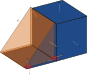
\includegraphics[width=.5\linewidth]{normal-criterion.png}
  \caption{Illustration of the \emph{Matching Normals Criterion}: The orange patch hull (drawn at an offset) is being tested for validity. For two hull facets and two mesh faces, the normals of the hull do not match the mesh normals. The mismatches are indicated in red.}
  \label{fig:matching-normals}
\end{figure}

See figure~\ref{fig:matching-normals}.

\subsubsection{Boundary Constraint Bars Criterion}

\subsubsection{Touching Triangles on Negative Side Criterion}

\subsection{Merge Cost}

\subsection{Flat Patches}

\subsection{Optimisations}

\subsubsection{Spatial Indices}

As mentioned in Section~\ref{}, the merge criteria within the patch validity computation involve predicates over all vertices, edges and faces of the input mesh. However, only predicate results computed on mesh features that spatially close to the patch feature in question actually contribute to the result. For this reason, the computation can be restricted to such mesh features from the beginning by querying spatial indices which support efficient spatial queries for mesh features. We use a modified kd-tree~\cite{} which supports AABB intersection queries TODO explain.

\subsubsection{Priority Queue for Merging}

Cite implementation? Describe cost to integer conversion?

\section{Extensions}\label{extensions}

\subsection{Parallelisation}

\begin{itemize}
\item Initial computation of index structures is parallelized using \texttt{laparallel:plet}: vertex, edge and face indices as well as boundary edge index
\item When two patches are merged, new patch links with the new patch at one end of the link are generated which requires expensive computations for evaluating the validity of the merged patch as well as computing the convex hull of the merged.
\end{itemize}

\subsection{Merge Tolerance}

\section{Results}\label{results}

Illustration of some generic results

Illustration of ``tolerance''?

Run times for some input meshes?

\section{Conclusion}\label{conclusion}


\section{Further Work}\label{further-work}


\section{Acknowledgements}\label{acknowledgements}


\bibliography{paper}

\end{document}

%%% Local Variables:
%%% mode: latex
%%% TeX-command-extra-options: "-shell-escape"
%%% TeX-master: t
%%% TeX-engine: luatex
%%% End:
